%!TEX root = ../Masterthesis.tex
\chapter{System perquisites}

Before elaborating a final system conception, some perquisites have to be defined.

System components to be defined:
\begin{itemize}
 \item Display hardware
 \item Tracking Technology
 \item Tracking Hardware
 \item Data cleaning
 \item Image analysis
 \item Data cleaning
 \item Inverse kinematics algorithm
 \item Hand model
 \end{itemize} 

 \section{Display}
 The first definition that has to be done is actually the last component of the processing chain. The final display hardware properties have to be defined initially as these are the determining factor for all other components. Since the goal of hand and object tracking is the most immersive when using a virtual reality headset rather than a normal display, these do not need to be taken into consideration.\\
Another device category which may be in the focus of interest are current mobile device platforms like \textit{Google cardboard} or the \textit{Samsung Gear} platform. In terms of creating an low cost consumer grade solution, these devices should be the first category to look at, as they are more widely available and do not need extra hardware except the smart-phone. Most modern devices have native support of WebGL in the browser and the emerging \textit{WebXR} Standard makes it fairly easy to display VR content. They also come with the convenience of already having a set of integrated sensors for position an rotation integrated. The downside of this device class reveals when taking a look at the hardware specifications of these devices. Although the newest high tier consumer grade devices do have a good performance output for their size they are still no comparison for a desktop setup. Also these devices, as they are first of all mobile phones, show lacks for wire connections, making it necessary to mostly communicate over wireless protocols. This leads to a growth in infrastructure(server, wi-fi-hotspot, etc.) and every further node in the processing chain leads to a physical signal delay.\\
After these first preliminary steps, only pure VR-Headsets like the \textit{HTC Vive}\cite{HTC.2018}or \textit{Occulus Rift} \cite{OculusVR.2018}should be the main focus. These headsets also provide the capabilities of motion tracking while utilizing the processing capabilities of a dedicated GPU and high-power CPU capabilities of modern desktop computers. Furthermore, they provide a variety of connection ports for wired connections, eliminating the need for wireless transmissions. In terms of cost, these devices do lie on the more costly side as you need the headset itself and a hardware setup which is capable of providing the output frame rate needed. But with the latest generations of GPU's and CPU's, this category was opened towards the normal consumer.\\
The \textit{HTC Vive} as well as the \textit{Occulus Rift} are able to display 90 images per second on their displays with each having a resolution of 2160x1200 pixels, resulting in a little over full HD resolution per eye. The duration of one frame is therefore around 11 ms. This is the time frame in which the rest of the components can theoretically supply the image data, do the image analysis to retrieve the tracking data, recalculate the IK model, calculate the object position and render the whole scene before sending it to the headset to be displayed.
\section{Tracking technology}
Physical sensors placed on the hand tend to give more precise tracking results compared to optical methods. The cost for the data precision is that the sensors have to be mounted to the hand in some kind of fashion. Cables or fibers, depending on sensor type, can hinder the hand movement. Utilizing  a glove based system brings the downside of the " one size fits all" problem. Human hands can differ largely in size, therefore on glove will not be able to be used for a wide range of users. Furthermore cloth gloves tend to get dirty while usage and are therefore unsuitable in therms of hygiene.\\

Color markers can be utilized very easily. The simplest form could be colored electrical tape wrapped around the fingertips. These markers can be made disposable after usage. The size of the marker can be adapted to be large enough to realize a robust tracking while being small enough to not constrain hand movement. They also provide the possibility to perform a person specific calibration of the hand model in an initialization step.
The easiest way to detect color markers is to use an optical tracking system.
Monocular optical tracking system are relatively easy to set up as they only need one camera, the complexity in the later processing steps of evaluating the marker positions from  only a single frame rises drastically.\\
Stereoscopic system in comparison have a higher initial effort in setting up and calibrating the system, but the further processing steps are fairly easy. 

\section{Tracking Hardware}
 As explained int the previous chapters, the motion of the human hand can be complex and in some cases really fast. Therefore, the optical tracking hardware should ideally be able to record images with the same or higher frequency as the display medium that is to be used. Prosumer and professional grade cameras are theoretically able to produce these kind of frame rates (60 fps and above), but most of the time store these high frame-rate videos directly to a hard drive rather than broadcasting them somewhere. Also the hardware that is needed to record such specific high frame rates is relatively expensive. Consumer grade cameras like the GoPro that are affordable, can record at a frame-rate of 120 fps but the live transmission of this material has a time lack of several frames.\\
\\When trying to utilize low cost hardware the limitation of recording and sending a video signal from a camera to a processing hardware will therefore be limited to 60fps. This process would also introduce further latency on the transport and would force a further reduction of frame rate to satisfy the time frame given by the display frame rate.
\\Another option that can be taken into consideration is to completely eliminate the need to transport the image data from camera to another device. This can be achieved when the camera and the computational hardware are located on the same hardware.\\The \textit{Raspberry Pi 3} microcomputer, which comes from the \textit{internet of things} world provides this capability. It combines a quite powerful computation capacity with an on-board hardware connector for a camera. The camera hardware is able to record in a FullHD resolution at 60fps and at lower resolutions up to 90fps. The camera module is directly connected on the the circuitboard, providing direct access for further processing.\\
For a complete 3 dimension space tracking, a one camera setup is not sufficient as it lack the data for the depth position of the object. To get this data, further hardware is needed. One option would be the utilization of a time of flight based depth sensing system like the ones described in Section \ref{sec:state_of_the_art}, but these system do come at a rather high entry level price.
\\Another option could be the tracking  pods that HTC offers as an expansion to it's time of flight \textit{Vive} system. These trackers could provide 3D positional data but with the downside of being relatively bulky. This would hinder the movement space of the hand and the tracker would have to be positioned on the arm as near as possible to the wrist. This would result in the position of only the wrist and not providing data on each individual finger of the hand. But as hindering as these trackers are on the hand, they could be easily used to provide tracking data for used objects.The tracker could be positioned onto the object where it does not hinder the usage. \\
Since the hardware setup of the Raspberry Pi with the camera is relatively easy and cost efficient, the usage of a second Raspberry Pi with a camera is good leverage point. The two cameras can be setup to create a stereoscopic camera setup which provides information about depth position through the disparity of the two camera images. 
Furthermore the image operations that need to be independently applied to each of the cameras frames can be done on the two separate device, eliminating the need for sending data traffic with image information through the network for post processing.
\\Downside of this method is that with all stereoscopic camera setups, the two cameras need to have some kind of frame synchronization to get the right two frames for evaluation.
\section{Data Filtering}
Every system that deals with the computation of live data is suspect to data fluctuation in input and output values. It is also to be assumed that the system will not be able to achieve an ideal synchronization between the cameras. This will probably introduce a degradation of tracking performance which has to be handled. It has to be evaluated at which point a data filtering will lead to the best end results.
\section{Image analysis}
The images recorded by the camera system need to be processed further down the line to get the positional data of selected hand features. The most common library to do such kinds of image processing is the \textit{OpenCV}\cite{OpenCVTeam.2018} library which is originally written in C and was ported into several other programming languages. It has build in features for camera calibration, color and object detection as well as several image optimization features that might be helpful for the processing.
\section{Inverse kinematics}
The inverse kinematics model is the second essential part of the setup after the tracking hardware. It receives the position data from the image post-processing and calculates the resulting current hand model position. The applied algorithm for the IK solution should be able to keep up with the data-flow from the tracking algorithm and should produce a fluid optical result on the display. As the calculation of the IK solution and the rendering of the scene with the models should be done on the same machine, computation power and memory consumption should be critical criteria. As the system will rely on optical tracking data, an algorithm that is capable of dealing with tracker occlusions and recovery from this data loss should be prioritized.
\newpage
\section{Hand model}
After retrieving all needed data from the real world counterpart and calculation for pose estimation is finished, the returned solution has to be displayed in the digital world. Therefore a digital hand model is needed to represent the calculated data. Modern day computer animation techniques make it possible to create nearly photo realistic digital replicas of human skin wrapped onto anatomically precisely modeled body parts. These highly complex models acquire a lot of calculation resources and are mostly not appropriate for a mealtime rendering approach.\\
When adapting calculation data to digital hand models, those of lesser complexity are preferred, sacrificing the quality of the resulting output for speed and more fluent motion results.
\begin{figure}[H]
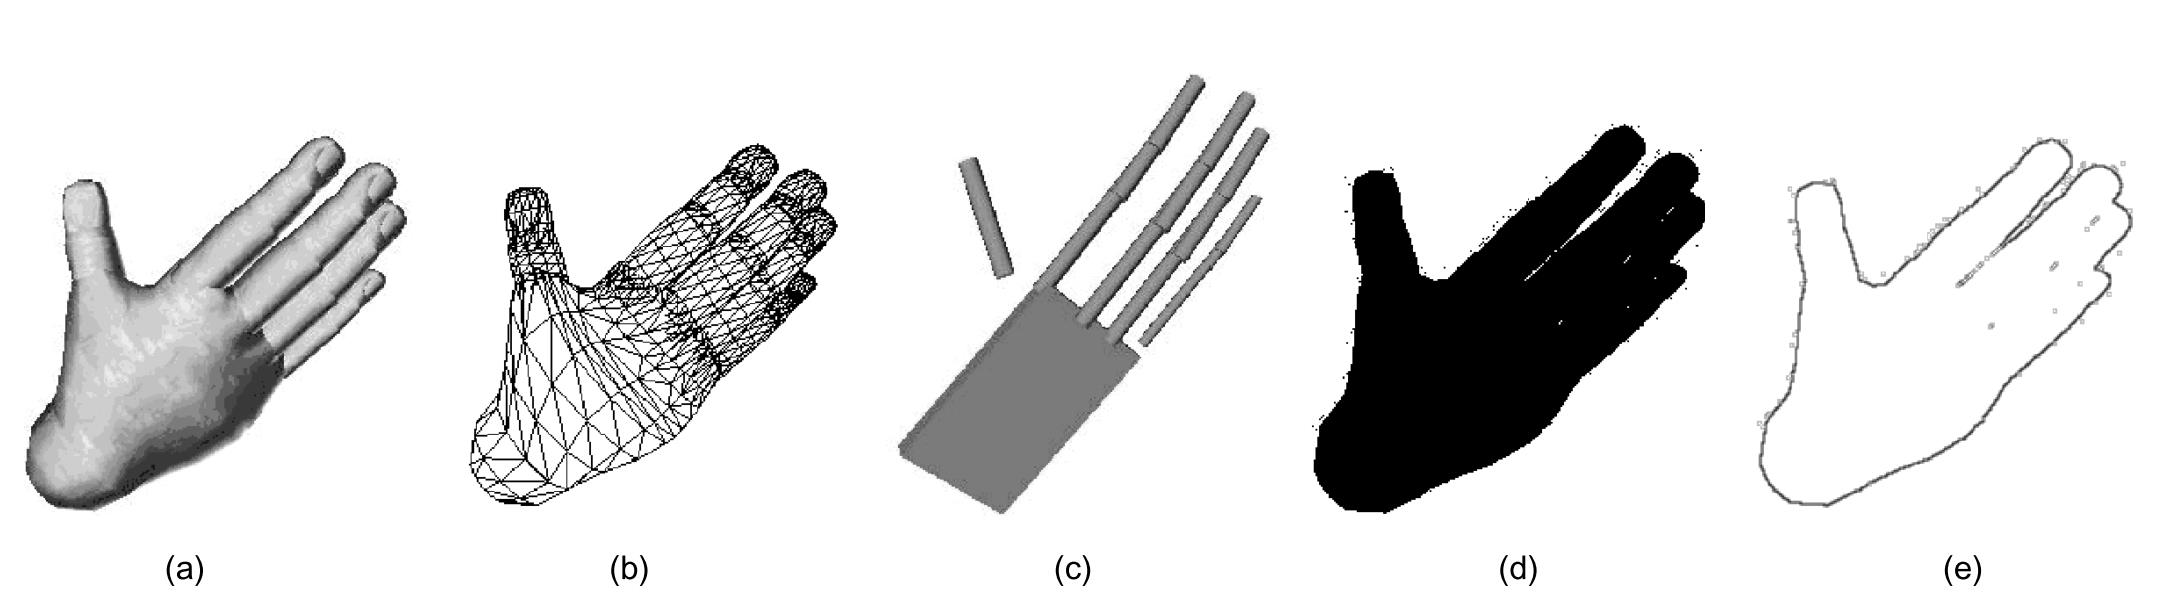
\includegraphics[width=\textwidth]{images/Pavlovic-Sharmaetal.jpg}
\caption{Pavlovic, Sharma et al: Hand models. Different hand models can be used to represent the same hand posture. (a) 3D Textured volumetric model. (b) 3D wire frame volumetric model. (c) 3D skeletal model. (d) Binary silhouette. (e) Contour.}
~\cite[p.~682]{Pavlovic.1997}
\label{handmodels_detail_level}
\end{figure}
Figure \ref{handmodels_detail_level} shows different model representations of the same hand posture. The models of \textbf{(a)}and \textbf{(b)} represent the aforementioned types of models that would be used in modern computer-graphics for displaying hand models realistically.\\These models are based on complex 3D surfaces like \textit{NURBS}(nonuniform rational B-splines) which are wrapped around an underlying skeleton. The wire frame model of \textbf{(b)} give a good overview of how many vertex calculation have to be made for the surface in each frame, causing these models to hardly run in real time if not supplying a large amount of computational power.\\
In applications where the 3D orientation of each individual finger is not necessary for processing and the general silhouette is sufficient (e.g general hand position tracking or sign language detection), even more reduced representation forms like \textbf{(d)} and \textbf{(e)} can be chosen.
The model displayed in \textbf{(c)} is a simplification of the human hand structure with geometric primitives like cylinders and boxes. These geometric primitives have the virtue of being much easier to describe than a \textit{NURBS} model. A cylinder for example is fully described by its height and its radius under the assumption that the position and orientation data is generally needed for all the described models.This type of model is also refereed to as \textit{skeletal models} as they mostly try to reproduce the strucutre of the human hand as described in Section \ref{sec:Physiological_structure_of_the_human_hand}.\\
For evaluation purposes, a rather simple model form should be used for the representation of the tracked hand in the digital space. The outcome results for tracking accuracy, update speed and the resulting match of physical and digital position of the hand are of more relevance than a highly realistic hand model.
\\To receive a correct optical result of the hand model finger and hand dimensions have to be measured for each hand specifically and stored into a data model for correct bone dimensions of the hand model. Ideally, this step should be automate-able and included into the system spin up process.
 